The methods seen approach the problem from a probabilistic point of view but, are not guaranteed, it relies on the probability of the robot to not be an outlier, and when we need a sure position of the robot it could lead to a failure (in a harmful environment or in interaction with humans it would be hazardous). The interval analysis means to guarantee the result, and is not subject to approximation because it does not need to linearise the problem. Interval Analysis has grown to be a competent alternative to the probabilistic methods.

\subsection{Interval Analysis}

In the Intervals theory a real number is replaced by an interval with an uncertainty represented by its width that includes the right number, for a known x the corresponding interval could be $[ \,x,-\epsilon,x+\epsilon] \,$ with a width of $2\epsilon$.

\begin{figure}[H]
\centering
    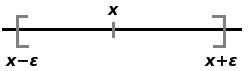
\includegraphics[scale=0.6]{Interval.png} 
    \caption{Representation of an interval.}
    \label{fig:interExample}
\end{figure}

This representation has advantages, to easily manage uncertainties by enclosing them in an interval, but the intervals can be contracted around the feasible value thus reducing the uncertainty.\\

This representation have advantages, to easily manage uncertainties by enclosing them in an interval, but the intervals can be contracted around the feasible value thus reducing the uncertainty.\\
For example considering the sets $X=[\,1,7]\,$ and $Y=[\,-1,5]\,$ and if $Y$ and $X$ are constraint by the equation $y=x^{2}$ then we can contract the set $Y$:\\

$Y = Y\cap X^{2} =[\,1,5]\,$\\

But X can also be contracted by going backwards:\\

$X=X\cap \sqrt{Y} =[\,0,\sqrt{5}]\,$\\

This operation is a forward-backward contractor ~\cite{jaulin2001applied}.

\begin{figure}[H]
\centering
    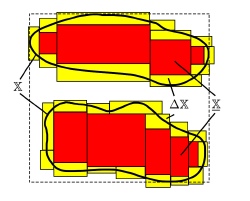
\includegraphics[scale=0.6]{subpaving.png} 
    \caption{Sub paving of a 2 dimensional set \cite{Bet14}.}
    \label{fig:subExample}
\end{figure}


The set inversion \cite{jaulin1993set}, finding $X$ such as $f([\,X]\,)$ is in S, is easy to compute with intervals' arithmetic if X is the solution set (see above, the red boxes are included in the set, yellow boxes are on the border), the minimal size of the boxes correspond to the precision for the set inversion.\\ 
One of the first papers to address the SLAM problem via interval analysis was in \cite{di2004set}, in this paper they proposed an algorithm for the mapping and localization using landmarks.

\begin{figure}[H]
\centering
    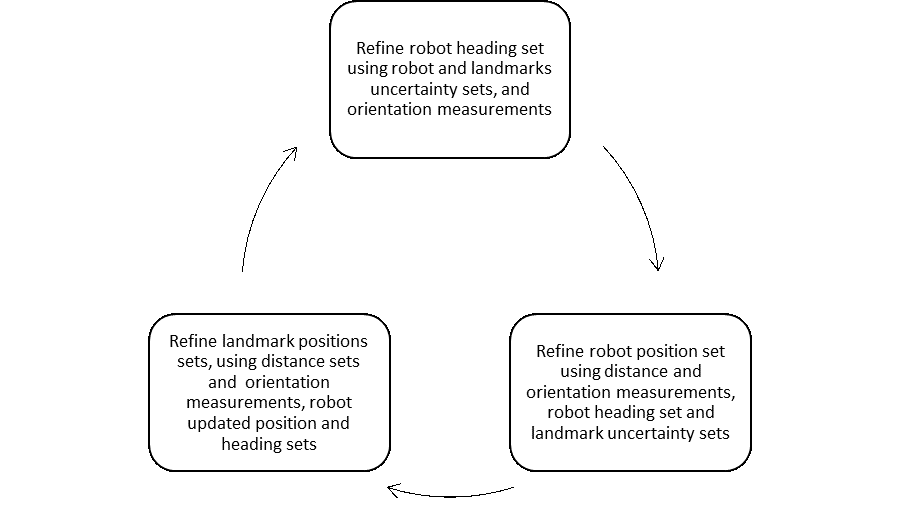
\includegraphics[scale=0.7]{algoslam.png} 
    \caption{Algorithm process for the SLAM \cite{di2004set}.}
    \label{fig:algoslamExample}
\end{figure}

In their case, figure 7, they considered receiving bearing and distance of landmarks, by using constraints propagation (contractors) we can refine the sets \cite{jaulin2010resolution}

\begin{figure}[H]
\centering
    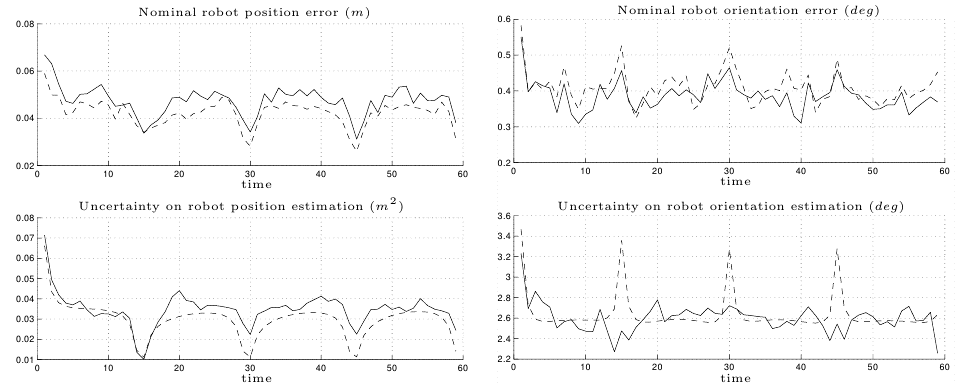
\includegraphics[scale=0.9]{difalgo.png} 
    \caption{Error differences between EKF-SLAM and Interval SLAM in \cite{di2004set}.}
    \label{fig:difalgo}
\end{figure}

The interval method can be as precise as the EKF-SLAM but with having a guaranteed uncertainty.